\newpage
\section[Исследование распределения Больцмана]{Исследование распределения Больцмана}

Начальные параметры (нормальные условия при $h = 0$, концентрация $n_{0}$ равна постоянной Лошмидта):
\begin{center}
    \begin{tabular}{c}
    \begin{lstlisting}
(*Constants*)
R = 8.31445985; (*The gas constant*)
g = 9.8066; (*Acceleration*)
n0 = 2.68678112*10^25; (*Loschmidt constant*)

(*Molar mass*)
H2M = 2;
N2M = 26;
O2M = 32;
AirM = 29;
    \end{lstlisting}
    \end{tabular}
\end{center}

Функции изменения температуры с высотой ($T_{0}$ постоянна, $T_{1}$ убывает с увеличением высоты, достигая значения 0):
\begin{equation*}
    \begin{gathered}
        T_{0}(h) = 273.15K = const\\
        T_{1}(h) = T_{0} - 6.5h
    \end{gathered}
\end{equation*}

Листинг программы Mathemtica:
\begin{center}
    \begin{tabular}{c}
    \begin{lstlisting}
 (*Temperature*)
T0[h_] = 273.15;
T1[h_] = Piecewise[{{T0[0] - 6.5 * h, T0[0] >= 6.5 * h},
                    {0, T0[0] < 6.5 * h}}];
    \end{lstlisting}
    \end{tabular}
\end{center}

Распределение Больцмана ($\mu$ --- молярная масса газа):
\begin{equation*}
    n(h) = n_{0} \cdot exp(-\frac{\mu  gh}{RT})
\end{equation*}


Листинг программы Matematica (\textbf{Plot} для $T_{0}$, для $T_{1}$ аналогично):
\begin{center}
    \begin{tabular}{c}
    \begin{lstlisting}
(*Boltzmann distribution*)
n[h_, M_, T_] = n0*Exp[-M*g*h/(R*T)];

Plot[{n[h, H2M, T0[h]],
      n[h, N2M, T0[h]],
      n[h, O2M, T0[h]],
      n[h, AirM, T0[h]]},
     {h, 0, 50},
     PlotLegends -> "Expressions",
     AxesLabel -> {h, n[h]}]
    \end{lstlisting}
    \end{tabular}
\end{center}


Полученные графики распределения Больцмана:
\hspace{0pt}
\begin{figure}[H]
    \centering
    \begin{minipage}[h]{0.8\linewidth}
        \center{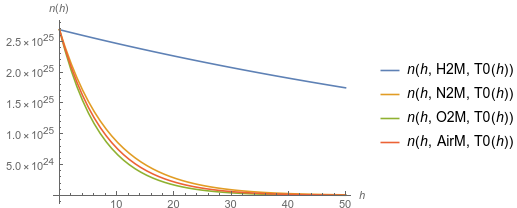
\includegraphics[width=1\linewidth]{2_1_boltz_t_const.png}}\\
        $T=T_{0}(h)=const$
    \end{minipage}
    \vfill
    \vspace{6pt}
    \begin{minipage}[h]{0.8\linewidth}
        \center{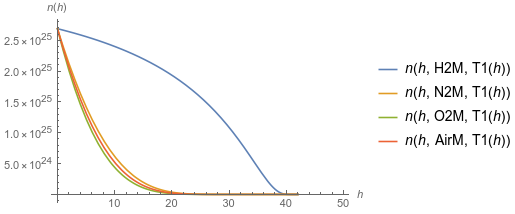
\includegraphics[width=1\linewidth]{2_2_boltz_t_change.png}}\\
        $T=T_{1}(h) \neq const$
    \end{minipage}
\end{figure}
